\documentclass[11pt,preprint, authoryear]{elsarticle}

\usepackage{lmodern}
%%%% My spacing
\usepackage{setspace}
\setstretch{1.2}
\DeclareMathSizes{12}{14}{10}{10}

% Wrap around which gives all figures included the [H] command, or places it "here". This can be tedious to code in Rmarkdown.
\usepackage{float}
\let\origfigure\figure
\let\endorigfigure\endfigure
\renewenvironment{figure}[1][2] {
    \expandafter\origfigure\expandafter[H]
} {
    \endorigfigure
}

\let\origtable\table
\let\endorigtable\endtable
\renewenvironment{table}[1][2] {
    \expandafter\origtable\expandafter[H]
} {
    \endorigtable
}


\usepackage{ifxetex,ifluatex}
\usepackage{fixltx2e} % provides \textsubscript
\ifnum 0\ifxetex 1\fi\ifluatex 1\fi=0 % if pdftex
  \usepackage[T1]{fontenc}
  \usepackage[utf8]{inputenc}
\else % if luatex or xelatex
  \ifxetex
    \usepackage{mathspec}
    \usepackage{xltxtra,xunicode}
  \else
    \usepackage{fontspec}
  \fi
  \defaultfontfeatures{Mapping=tex-text,Scale=MatchLowercase}
  \newcommand{\euro}{€}
\fi

\usepackage{amssymb, amsmath, amsthm, amsfonts}

\def\bibsection{\section*{References}} %%% Make "References" appear before bibliography


\usepackage[round]{natbib}

\usepackage{longtable}
\usepackage[margin=2.3cm,bottom=2cm,top=2.5cm, includefoot]{geometry}
\usepackage{fancyhdr}
\usepackage[bottom, hang, flushmargin]{footmisc}
\usepackage{graphicx}
\numberwithin{equation}{section}
\numberwithin{figure}{section}
\numberwithin{table}{section}
\setlength{\parindent}{0cm}
\setlength{\parskip}{1.3ex plus 0.5ex minus 0.3ex}
\usepackage{textcomp}
\renewcommand{\headrulewidth}{0.2pt}
\renewcommand{\footrulewidth}{0.3pt}

\usepackage{array}
\newcolumntype{x}[1]{>{\centering\arraybackslash\hspace{0pt}}p{#1}}

%%%%  Remove the "preprint submitted to" part. Don't worry about this either, it just looks better without it:
\makeatletter
\def\ps@pprintTitle{%
  \let\@oddhead\@empty
  \let\@evenhead\@empty
  \let\@oddfoot\@empty
  \let\@evenfoot\@oddfoot
}
\makeatother

 \def\tightlist{} % This allows for subbullets!

\usepackage{hyperref}
\hypersetup{breaklinks=true,
            bookmarks=true,
            colorlinks=true,
            citecolor=blue,
            urlcolor=blue,
            linkcolor=blue,
            pdfborder={0 0 0}}


% The following packages allow huxtable to work:
\usepackage{siunitx}
\usepackage{multirow}
\usepackage{hhline}
\usepackage{calc}
\usepackage{tabularx}
\usepackage{booktabs}
\usepackage{caption}


\newenvironment{columns}[1][]{}{}

\newenvironment{column}[1]{\begin{minipage}{#1}\ignorespaces}{%
\end{minipage}
\ifhmode\unskip\fi
\aftergroup\useignorespacesandallpars}

\def\useignorespacesandallpars#1\ignorespaces\fi{%
#1\fi\ignorespacesandallpars}

\makeatletter
\def\ignorespacesandallpars{%
  \@ifnextchar\par
    {\expandafter\ignorespacesandallpars\@gobble}%
    {}%
}
\makeatother

\newenvironment{CSLReferences}[2]{%
}

\urlstyle{same}  % don't use monospace font for urls
\setlength{\parindent}{0pt}
\setlength{\parskip}{6pt plus 2pt minus 1pt}
\setlength{\emergencystretch}{3em}  % prevent overfull lines
\setcounter{secnumdepth}{5}

%%% Use protect on footnotes to avoid problems with footnotes in titles
\let\rmarkdownfootnote\footnote%
\def\footnote{\protect\rmarkdownfootnote}
\IfFileExists{upquote.sty}{\usepackage{upquote}}{}

%%% Include extra packages specified by user
\usepackage{array}
\usepackage{caption}
\usepackage{graphicx}
\usepackage{siunitx}
\usepackage[normalem]{ulem}
\usepackage{colortbl}
\usepackage{multirow}
\usepackage{hhline}
\usepackage{calc}
\usepackage{tabularx}
\usepackage{threeparttable}
\usepackage{wrapfig}
\usepackage{adjustbox}
\usepackage{hyperref}

%%% Hard setting column skips for reports - this ensures greater consistency and control over the length settings in the document.
%% page layout
%% paragraphs
\setlength{\baselineskip}{12pt plus 0pt minus 0pt}
\setlength{\parskip}{12pt plus 0pt minus 0pt}
\setlength{\parindent}{0pt plus 0pt minus 0pt}
%% floats
\setlength{\floatsep}{12pt plus 0 pt minus 0pt}
\setlength{\textfloatsep}{20pt plus 0pt minus 0pt}
\setlength{\intextsep}{14pt plus 0pt minus 0pt}
\setlength{\dbltextfloatsep}{20pt plus 0pt minus 0pt}
\setlength{\dblfloatsep}{14pt plus 0pt minus 0pt}
%% maths
\setlength{\abovedisplayskip}{12pt plus 0pt minus 0pt}
\setlength{\belowdisplayskip}{12pt plus 0pt minus 0pt}
%% lists
\setlength{\topsep}{10pt plus 0pt minus 0pt}
\setlength{\partopsep}{3pt plus 0pt minus 0pt}
\setlength{\itemsep}{5pt plus 0pt minus 0pt}
\setlength{\labelsep}{8mm plus 0mm minus 0mm}
\setlength{\parsep}{\the\parskip}
\setlength{\listparindent}{\the\parindent}
%% verbatim
\setlength{\fboxsep}{5pt plus 0pt minus 0pt}



\begin{document}



\begin{frontmatter}  %

\title{Question 3: Coldplay vs Metallica}

% Set to FALSE if wanting to remove title (for submission)




\author[Add1]{Grace Grant}
\ead{21653488@sun.ac.za}





\address[Add1]{Stellenbosch University, Stellenbosch, South Africa}



\vspace{1cm}


\begin{keyword}
\footnotesize{
Multivariate GARCH \sep Kalman Filter \sep Copula \\
\vspace{0.3cm}
}
\footnotesize{
\textit{JEL classification} L250 \sep L100
}
\end{keyword}



\vspace{0.5cm}

\end{frontmatter}

\setcounter{footnote}{0}



%________________________
% Header and Footers
%%%%%%%%%%%%%%%%%%%%%%%%%%%%%%%%%
\pagestyle{fancy}
\chead{}
\rhead{}
\lfoot{}
\rfoot{\footnotesize Page \thepage}
\lhead{}
%\rfoot{\footnotesize Page \thepage } % "e.g. Page 2"
\cfoot{}

%\setlength\headheight{30pt}
%%%%%%%%%%%%%%%%%%%%%%%%%%%%%%%%%
%________________________

\headsep 35pt % So that header does not go over title




\hypertarget{introduction}{%
\section{Introduction}\label{introduction}}

Coldplay and Metallica are two of the longest-lasting bands of this
generation, with careers spanning more than two decades. The following
report outlines some of the interesting factors associated with each
band's popularity, making use of graphics to illustrate the results.

\hypertarget{danceability}{%
\section{Danceability}\label{danceability}}

Everybody loves to dance when listening to music as a form of outlet and
a way to have fun. This table shows the top 10 songs based on
danceability according to Spotify. Many of these artists are highly
successful, indicating a possible link between danceability and
popularity.

 
  \providecommand{\huxb}[2]{\arrayrulecolor[RGB]{#1}\global\arrayrulewidth=#2pt}
  \providecommand{\huxvb}[2]{\color[RGB]{#1}\vrule width #2pt}
  \providecommand{\huxtpad}[1]{\rule{0pt}{#1}}
  \providecommand{\huxbpad}[1]{\rule[-#1]{0pt}{#1}}

\begin{table}[ht]
\begin{centerbox}
\begin{threeparttable}
 \label{tab:unnamed-chunk-1}
\setlength{\tabcolsep}{0pt}
\begin{tabular}{l l l}


\hhline{>{\huxb{0, 0, 0}{1}}->{\huxb{0, 0, 0}{1}}->{\huxb{0, 0, 0}{1}}-}
\arrayrulecolor{black}

\multicolumn{1}{!{\huxvb{0, 0, 0}{1}}l!{\huxvb{0, 0, 0}{1}}}{\huxtpad{6pt + 1em}\raggedright \hspace{6pt} {\fontsize{12pt}{14.4pt}\selectfont name} \hspace{6pt}\huxbpad{6pt}} &
\multicolumn{1}{l!{\huxvb{0, 0, 0}{1}}}{\huxtpad{6pt + 1em}\raggedright \hspace{6pt} {\fontsize{12pt}{14.4pt}\selectfont artist} \hspace{6pt}\huxbpad{6pt}} &
\multicolumn{1}{r!{\huxvb{0, 0, 0}{1}}}{\huxtpad{6pt + 1em}\raggedleft \hspace{6pt} {\fontsize{12pt}{14.4pt}\selectfont danceability} \hspace{6pt}\huxbpad{6pt}} \tabularnewline[-0.5pt]


\hhline{>{\huxb{0, 0, 0}{1}}->{\huxb{0, 0, 0}{1}}->{\huxb{0, 0, 0}{1}}-}
\arrayrulecolor{black}

\multicolumn{1}{!{\huxvb{0, 0, 0}{1}}l!{\huxvb{0, 0, 0}{1}}}{\huxtpad{6pt + 1em}\raggedright \hspace{6pt} {\fontsize{12pt}{14.4pt}\selectfont Leave Me Now} \hspace{6pt}\huxbpad{6pt}} &
\multicolumn{1}{l!{\huxvb{0, 0, 0}{1}}}{\huxtpad{6pt + 1em}\raggedright \hspace{6pt} {\fontsize{12pt}{14.4pt}\selectfont Herbert} \hspace{6pt}\huxbpad{6pt}} &
\multicolumn{1}{r!{\huxvb{0, 0, 0}{1}}}{\huxtpad{6pt + 1em}\raggedleft \hspace{6pt} {\fontsize{12pt}{14.4pt}\selectfont 0.986} \hspace{6pt}\huxbpad{6pt}} \tabularnewline[-0.5pt]


\hhline{>{\huxb{0, 0, 0}{1}}->{\huxb{0, 0, 0}{1}}->{\huxb{0, 0, 0}{1}}-}
\arrayrulecolor{black}

\multicolumn{1}{!{\huxvb{0, 0, 0}{1}}l!{\huxvb{0, 0, 0}{1}}}{\huxtpad{6pt + 1em}\raggedright \hspace{6pt} {\fontsize{12pt}{14.4pt}\selectfont Go Girl} \hspace{6pt}\huxbpad{6pt}} &
\multicolumn{1}{l!{\huxvb{0, 0, 0}{1}}}{\huxtpad{6pt + 1em}\raggedright \hspace{6pt} {\fontsize{12pt}{14.4pt}\selectfont Pitbull} \hspace{6pt}\huxbpad{6pt}} &
\multicolumn{1}{r!{\huxvb{0, 0, 0}{1}}}{\huxtpad{6pt + 1em}\raggedleft \hspace{6pt} {\fontsize{12pt}{14.4pt}\selectfont 0.985} \hspace{6pt}\huxbpad{6pt}} \tabularnewline[-0.5pt]


\hhline{>{\huxb{0, 0, 0}{1}}->{\huxb{0, 0, 0}{1}}->{\huxb{0, 0, 0}{1}}-}
\arrayrulecolor{black}

\multicolumn{1}{!{\huxvb{0, 0, 0}{1}}l!{\huxvb{0, 0, 0}{1}}}{\huxtpad{6pt + 1em}\raggedright \hspace{6pt} {\fontsize{12pt}{14.4pt}\selectfont Funky Cold Medina} \hspace{6pt}\huxbpad{6pt}} &
\multicolumn{1}{l!{\huxvb{0, 0, 0}{1}}}{\huxtpad{6pt + 1em}\raggedright \hspace{6pt} {\fontsize{12pt}{14.4pt}\selectfont Tone-Lōc} \hspace{6pt}\huxbpad{6pt}} &
\multicolumn{1}{r!{\huxvb{0, 0, 0}{1}}}{\huxtpad{6pt + 1em}\raggedleft \hspace{6pt} {\fontsize{12pt}{14.4pt}\selectfont 0.984} \hspace{6pt}\huxbpad{6pt}} \tabularnewline[-0.5pt]


\hhline{>{\huxb{0, 0, 0}{1}}->{\huxb{0, 0, 0}{1}}->{\huxb{0, 0, 0}{1}}-}
\arrayrulecolor{black}

\multicolumn{1}{!{\huxvb{0, 0, 0}{1}}l!{\huxvb{0, 0, 0}{1}}}{\huxtpad{6pt + 1em}\raggedright \hspace{6pt} {\fontsize{12pt}{14.4pt}\selectfont State of Shock} \hspace{6pt}\huxbpad{6pt}} &
\multicolumn{1}{l!{\huxvb{0, 0, 0}{1}}}{\huxtpad{6pt + 1em}\raggedright \hspace{6pt} {\fontsize{12pt}{14.4pt}\selectfont The Jacksons} \hspace{6pt}\huxbpad{6pt}} &
\multicolumn{1}{r!{\huxvb{0, 0, 0}{1}}}{\huxtpad{6pt + 1em}\raggedleft \hspace{6pt} {\fontsize{12pt}{14.4pt}\selectfont 0.982} \hspace{6pt}\huxbpad{6pt}} \tabularnewline[-0.5pt]


\hhline{>{\huxb{0, 0, 0}{1}}->{\huxb{0, 0, 0}{1}}->{\huxb{0, 0, 0}{1}}-}
\arrayrulecolor{black}

\multicolumn{1}{!{\huxvb{0, 0, 0}{1}}l!{\huxvb{0, 0, 0}{1}}}{\huxtpad{6pt + 1em}\raggedright \hspace{6pt} {\fontsize{12pt}{14.4pt}\selectfont Teachers} \hspace{6pt}\huxbpad{6pt}} &
\multicolumn{1}{l!{\huxvb{0, 0, 0}{1}}}{\huxtpad{6pt + 1em}\raggedright \hspace{6pt} {\fontsize{12pt}{14.4pt}\selectfont Daft Punk} \hspace{6pt}\huxbpad{6pt}} &
\multicolumn{1}{r!{\huxvb{0, 0, 0}{1}}}{\huxtpad{6pt + 1em}\raggedleft \hspace{6pt} {\fontsize{12pt}{14.4pt}\selectfont 0.98\hphantom{0}} \hspace{6pt}\huxbpad{6pt}} \tabularnewline[-0.5pt]


\hhline{>{\huxb{0, 0, 0}{1}}->{\huxb{0, 0, 0}{1}}->{\huxb{0, 0, 0}{1}}-}
\arrayrulecolor{black}

\multicolumn{1}{!{\huxvb{0, 0, 0}{1}}l!{\huxvb{0, 0, 0}{1}}}{\huxtpad{6pt + 1em}\raggedright \hspace{6pt} {\fontsize{12pt}{14.4pt}\selectfont Give It To Me} \hspace{6pt}\huxbpad{6pt}} &
\multicolumn{1}{l!{\huxvb{0, 0, 0}{1}}}{\huxtpad{6pt + 1em}\raggedright \hspace{6pt} {\fontsize{12pt}{14.4pt}\selectfont Timbaland} \hspace{6pt}\huxbpad{6pt}} &
\multicolumn{1}{r!{\huxvb{0, 0, 0}{1}}}{\huxtpad{6pt + 1em}\raggedleft \hspace{6pt} {\fontsize{12pt}{14.4pt}\selectfont 0.975} \hspace{6pt}\huxbpad{6pt}} \tabularnewline[-0.5pt]


\hhline{>{\huxb{0, 0, 0}{1}}->{\huxb{0, 0, 0}{1}}->{\huxb{0, 0, 0}{1}}-}
\arrayrulecolor{black}

\multicolumn{1}{!{\huxvb{0, 0, 0}{1}}l!{\huxvb{0, 0, 0}{1}}}{\huxtpad{6pt + 1em}\raggedright \hspace{6pt} {\fontsize{12pt}{14.4pt}\selectfont Ice Ice Baby (Radio Edit)} \hspace{6pt}\huxbpad{6pt}} &
\multicolumn{1}{l!{\huxvb{0, 0, 0}{1}}}{\huxtpad{6pt + 1em}\raggedright \hspace{6pt} {\fontsize{12pt}{14.4pt}\selectfont Vanilla Ice} \hspace{6pt}\huxbpad{6pt}} &
\multicolumn{1}{r!{\huxvb{0, 0, 0}{1}}}{\huxtpad{6pt + 1em}\raggedleft \hspace{6pt} {\fontsize{12pt}{14.4pt}\selectfont 0.975} \hspace{6pt}\huxbpad{6pt}} \tabularnewline[-0.5pt]


\hhline{>{\huxb{0, 0, 0}{1}}->{\huxb{0, 0, 0}{1}}->{\huxb{0, 0, 0}{1}}-}
\arrayrulecolor{black}

\multicolumn{1}{!{\huxvb{0, 0, 0}{1}}l!{\huxvb{0, 0, 0}{1}}}{\huxtpad{6pt + 1em}\raggedright \hspace{6pt} {\fontsize{12pt}{14.4pt}\selectfont Tape Song} \hspace{6pt}\huxbpad{6pt}} &
\multicolumn{1}{l!{\huxvb{0, 0, 0}{1}}}{\huxtpad{6pt + 1em}\raggedright \hspace{6pt} {\fontsize{12pt}{14.4pt}\selectfont The Kills} \hspace{6pt}\huxbpad{6pt}} &
\multicolumn{1}{r!{\huxvb{0, 0, 0}{1}}}{\huxtpad{6pt + 1em}\raggedleft \hspace{6pt} {\fontsize{12pt}{14.4pt}\selectfont 0.974} \hspace{6pt}\huxbpad{6pt}} \tabularnewline[-0.5pt]


\hhline{>{\huxb{0, 0, 0}{1}}->{\huxb{0, 0, 0}{1}}->{\huxb{0, 0, 0}{1}}-}
\arrayrulecolor{black}

\multicolumn{1}{!{\huxvb{0, 0, 0}{1}}l!{\huxvb{0, 0, 0}{1}}}{\huxtpad{6pt + 1em}\raggedright \hspace{6pt} {\fontsize{12pt}{14.4pt}\selectfont Heavy Machinery} \hspace{6pt}\huxbpad{6pt}} &
\multicolumn{1}{l!{\huxvb{0, 0, 0}{1}}}{\huxtpad{6pt + 1em}\raggedright \hspace{6pt} {\fontsize{12pt}{14.4pt}\selectfont Scuba} \hspace{6pt}\huxbpad{6pt}} &
\multicolumn{1}{r!{\huxvb{0, 0, 0}{1}}}{\huxtpad{6pt + 1em}\raggedleft \hspace{6pt} {\fontsize{12pt}{14.4pt}\selectfont 0.973} \hspace{6pt}\huxbpad{6pt}} \tabularnewline[-0.5pt]


\hhline{>{\huxb{0, 0, 0}{1}}->{\huxb{0, 0, 0}{1}}->{\huxb{0, 0, 0}{1}}-}
\arrayrulecolor{black}

\multicolumn{1}{!{\huxvb{0, 0, 0}{1}}l!{\huxvb{0, 0, 0}{1}}}{\huxtpad{6pt + 1em}\raggedright \hspace{6pt} {\fontsize{12pt}{14.4pt}\selectfont Long Shot Kick De Bucket} \hspace{6pt}\huxbpad{6pt}} &
\multicolumn{1}{l!{\huxvb{0, 0, 0}{1}}}{\huxtpad{6pt + 1em}\raggedright \hspace{6pt} {\fontsize{12pt}{14.4pt}\selectfont The Pioneers} \hspace{6pt}\huxbpad{6pt}} &
\multicolumn{1}{r!{\huxvb{0, 0, 0}{1}}}{\huxtpad{6pt + 1em}\raggedleft \hspace{6pt} {\fontsize{12pt}{14.4pt}\selectfont 0.971} \hspace{6pt}\huxbpad{6pt}} \tabularnewline[-0.5pt]


\hhline{>{\huxb{0, 0, 0}{1}}->{\huxb{0, 0, 0}{1}}->{\huxb{0, 0, 0}{1}}-}
\arrayrulecolor{black}
\end{tabular}
\end{threeparttable}\par\end{centerbox}

\end{table}
 

These scatter plots show the correlation between danceability and
popularity for each of the bands, indicating a positive link between the
two factors.

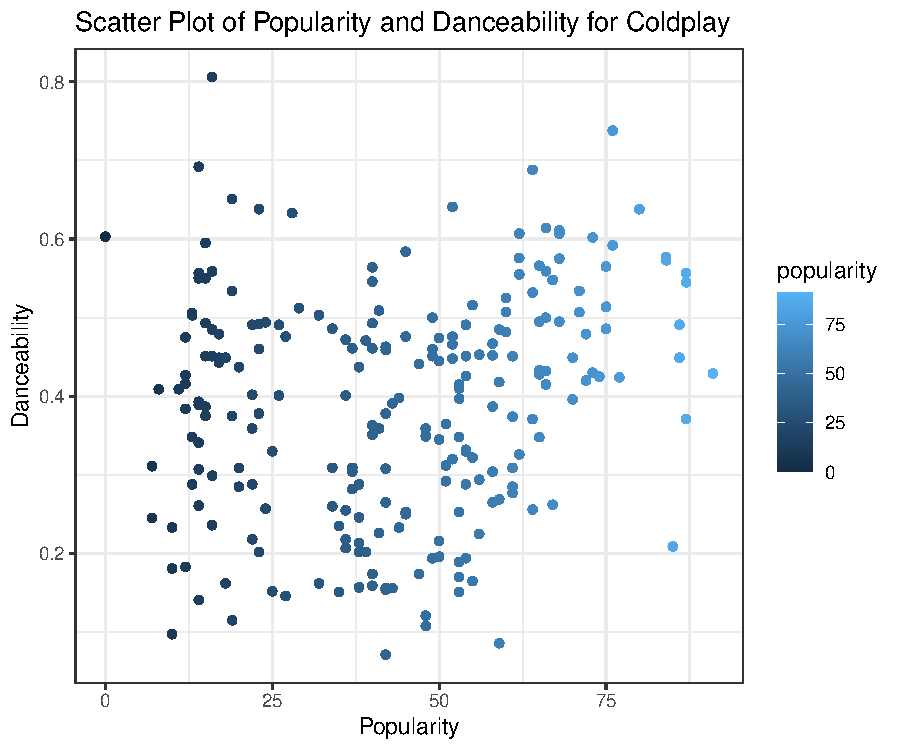
\includegraphics{Question-3_files/figure-latex/unnamed-chunk-2-1.pdf}

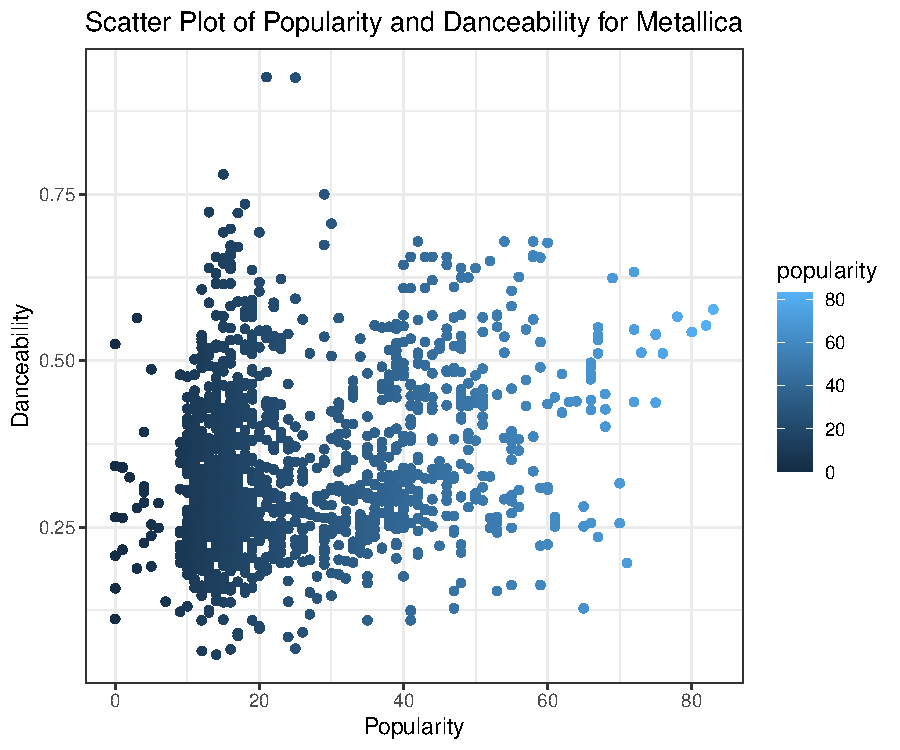
\includegraphics{Question-3_files/figure-latex/unnamed-chunk-3-1.pdf}

\hypertarget{popularity}{%
\section{Popularity}\label{popularity}}

The popularity of each of the bands' albums is also important to
consider and is highlighted in the following graphs.

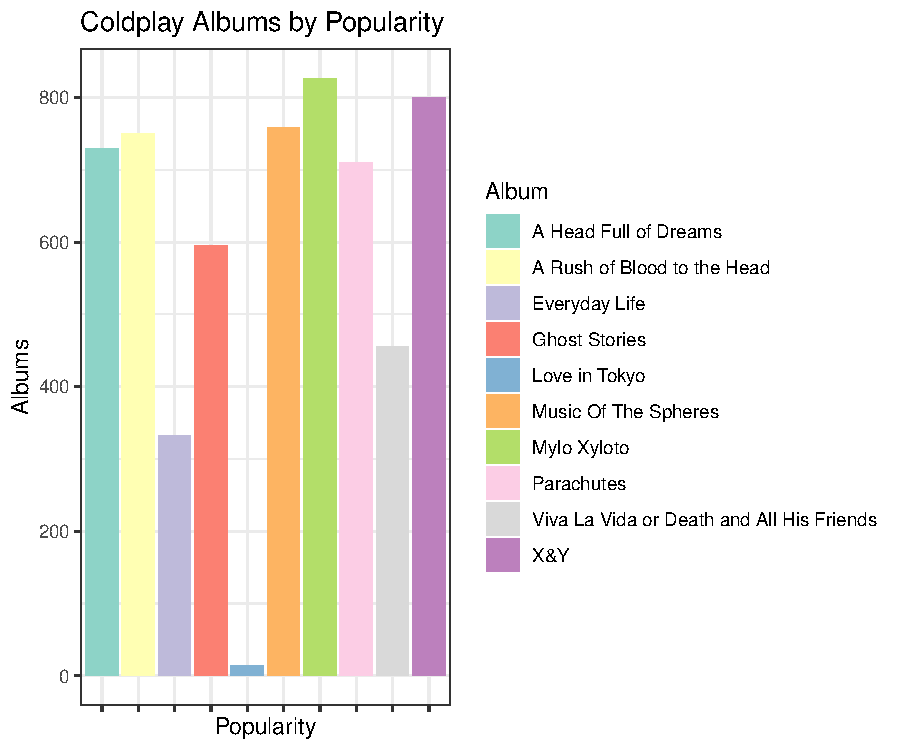
\includegraphics{Question-3_files/figure-latex/unnamed-chunk-4-1.pdf}

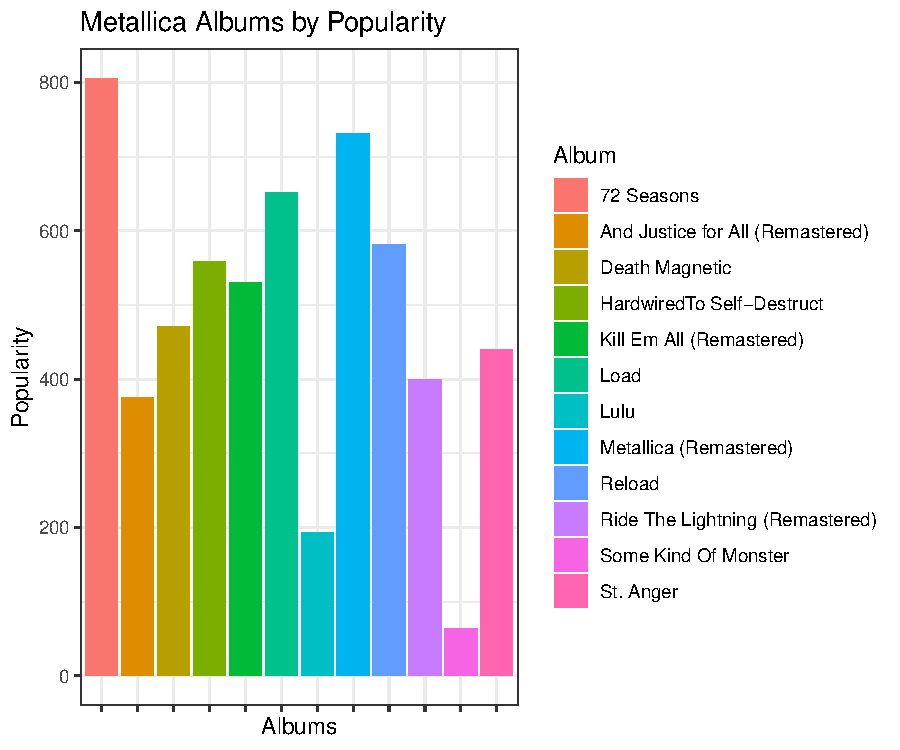
\includegraphics{Question-3_files/figure-latex/unnamed-chunk-5-1.pdf}

These graphs show that the most popular albums for Coldplay and
Metallica are Mylo Xyloto and 72 Seasons, respectively. The next set of
graphs also compares the popularity of each album but shows the
distribution across popularity by using box and whisker plots.

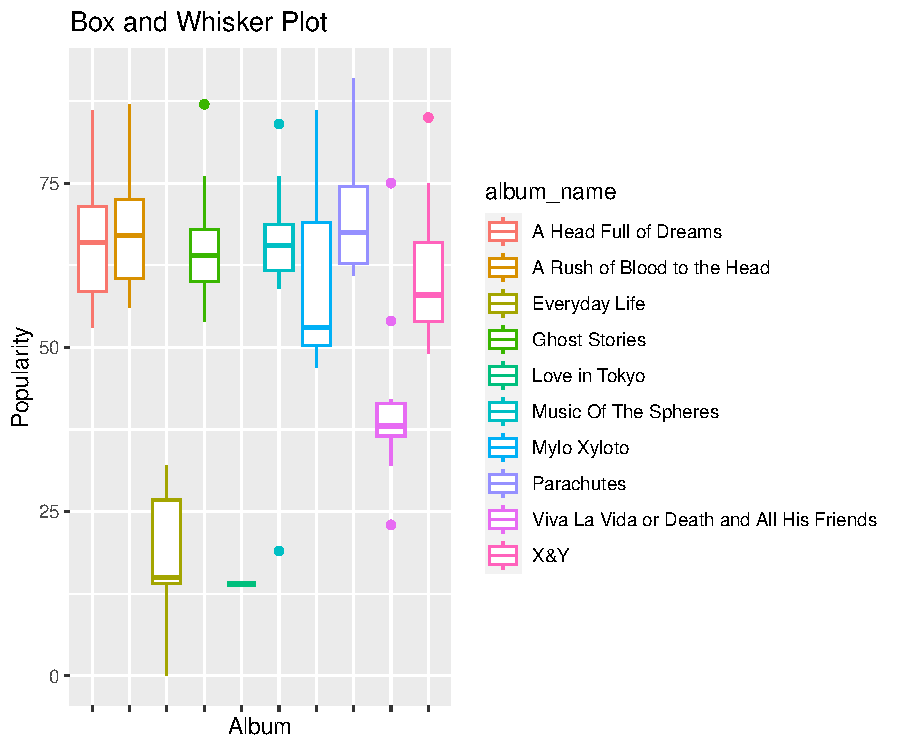
\includegraphics{Question-3_files/figure-latex/unnamed-chunk-6-1.pdf}

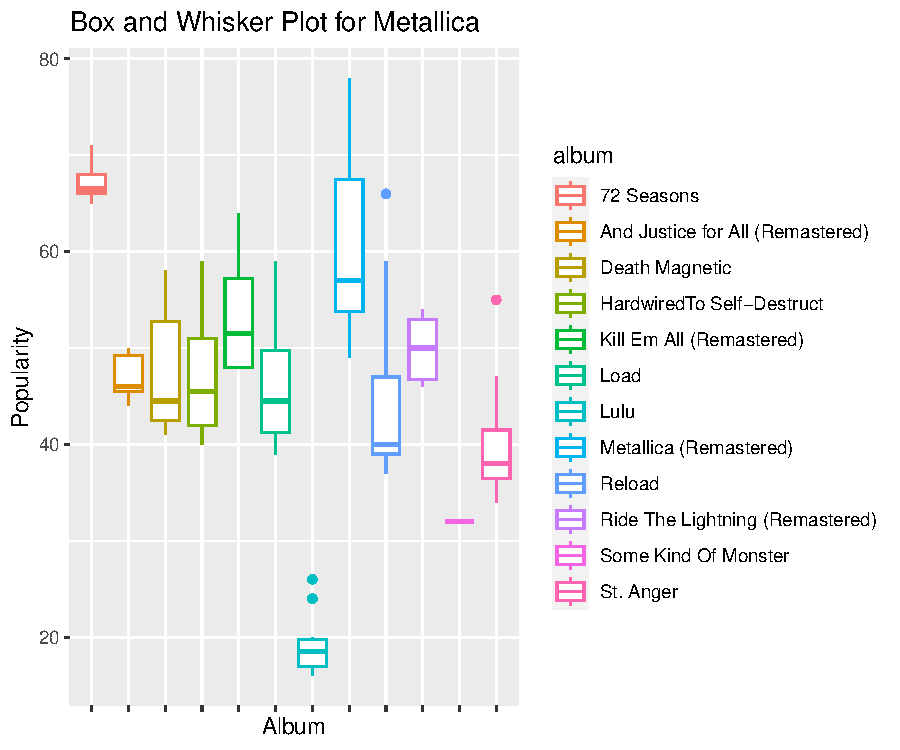
\includegraphics{Question-3_files/figure-latex/unnamed-chunk-7-1.pdf}

For some of the albums the distributions are quite large, indicating
greater diversity in the range of popularity perceptions for each album.
Considering the bands' most popular albums from the first bar graphs,
Mylo Xyloto and 72 Seasons, we see that Mylo Xyloto has a much more
spread out box and whisker plot compared to 72 Seasons. The latter album
can, therefore, be reliably considered as the most popular album for
Metallica. However, it may be better to consider A Head Full of Dreams
or Music of the Spheres as Coldplay's most popular albums as they have
smaller distributions while still having overall high popularity.

\bibliography{Tex/ref}





\end{document}
